% !TEX encoding = UTF-8
% !TEX TS-program = pdflatex
% !TEX root = ../tesi.tex

%**************************************************************
\chapter{Sviluppo del prototipo}
\label{cap:sviluppo-prototipo}
%**************************************************************

\intro{Questo capitolo illustra il funzionamento delle tecnologie che ho utilizzato nello sviluppo del prototipo, la logica di realizzazione ed il risultato ottenuto}\\

%**************************************************************
\section{AngularJS}
\label{sec:AngularJS}

La libreria che ho scelto di utilizzare, AngularJS, nasce nel 2012 nei laboratori di Google.\\
Esso potenzia l'aspetto dichiarativo del linguaggio \gls{html}, offrendo al contempo tutti gli strumenti necessari alla realizzazione di \gls{spag}. 
\subsection{Direttive e controller}
Una delle peculiarità di  AngularJS è che consente di aggiungere al codice HTML nuovi attributi, denominati \textbf{direttive}.\\
Tali direttive possono essere definite dall'utente, che comunque ha a disposizione anche un buon numero di 
direttive standard fornite dal \emph{framework}. Queste strutture consentono al compilatore HTML di AngularJS (attivate dal comando \lstinline[language=Java]!$compile()!, di creare un legame tra l'attributo in cui sono inserite ed il codice JavaScript che va ad eseguire il corpo della direttiva, tipicamente una funzione.\\
La possibilità di definire direttive customizzate estende di molto le funzionalità di base, lasciando alla fantasia del programmatore la creazione di strutture pensate appositamente per l'applicazione in sviluppo, ed consente di utilizzare quasi esclusivamente l'HTML per la creazione delle interfacce grafiche.\\
L'invocazione delle direttive può avvenire utilizzando il nome della direttiva come tag(\lstinline[language=HTML]!<direttiva></direttiva>!), oppure come attributo ad un tag regolare HTML(\lstinline[language=HTML]!<div direttiva></div>!).\\
Nel mio progetto ho utilizzato esclusivamente direttive standard di AngularJS, che ne ha create di specifiche per la creazione di form.\\
\\
L'altro importante componente di AngularJS è il controller. Esso viene invocato tramite la direttiva\lstinline[language=HTML]!ng-controller! ed il suo scope concerne tutto ciò che si trova all'interno dei tag nei quali è definito. Un controller, grazie al concetto di dependency injection, può utilizzare le funzionalità definite in moduli esterni che vengono inseriti come dipendenza all'interno del controller.\\ \'E possibile importare, oltre ad interi metodi, anche singoli oggetti: il più utilizzato è sicuramente l'oggetto di sistema  \lstinline[language=HTML]!$scope!. Quest'ultimo è un semplice oggetto JavaScript, per cui è possibile aggiungervi nuovi attributi e metodi semplicemente digitando \lstinline[language=HTML]!$scope.nuovoattributo = valore;!. Lo scope, assieme alle funzionalità definite nei moduli dichiarati come dipendenza, funge da \emph{model} nel patter MVC descritto in \ref{sec:MVC}.\\
Gli attributi dello \lstinline[language=HTML]!$scope! definiti in un controller sono condivisi all'interno della view (quindi nel codice HTML) unicamente nell'area in cui è definito il controller. AngularJS implementa infatti il concetto di \textbf{two-ways data binding}: il data binding è il meccanismo di sincronizzazione automatica dei dati tra il modello e la view. La maggior parte dei sistemi di template supporta il data binding in una sola direzione, tipicamente dal modello dei dati verso la view. Questo vuol dire che i dati del modello vengono combinati con il template HTML per generare la view visibile all’utente. Se però il modello viene modificato, le modifiche non si riflettono automaticamente sulla view. Analogamente, se l’utente modifica la view, queste modifiche non vengono automaticamente riportate sul modello dei dati. Per sincronizzare view e modello occorre in genere scrivere del codice che lo faccia.\\
Il data binding di AngularJS invece è bidirezionale, cioè ogni modifica al modello dei dati si riflette automaticamente sulla view e ogni modifica alla view viene riportata sul modello dei dati.\\
Per poter utilizzare un attributo dello \lstinline[language=HTML]!$scope! nella view è sufficiente indicarlo, all'interno di un tag di testo, con la seguente sintassi: \lstinline[language=Java]!{{nuovoattributo}}!. Questa sintassi, equivalente alla direttiva \lstinline[language=Java]!ng-model = nuovoattributo!, attiva il cosiddetto \emph{ciclo di digest}.

\subsection{Ciclo di digest}%TODO ciclo digest, watch, ng model
Il ciclo di digest è ciò che permette di avere il two ways data binding. Ogni volta che viene usata la sintassi \lstinline[language=Java]!{{nuovoattributo}}! o la sua equivalente, viene automaticamente creato un \textbf{watch} che ascolta i cambiamenti del valore della variabile a cui è associato, nel nostro caso la variabile "nuovoattributo".\\
Quando viene cambiato il valore di una variabile, il \emph{ciclo di digest} controlla tutti i watch presenti nell'applicazione e, nel caso verifichi il cambiamento di alcune variabili rispetto al ciclo precedente, esegue delle operazioni al fine di aggiornare il DOM nei punti in cui essa è utilizzata.\\
Nel caso di variabili che vengono modificate all'interno di un watch, ad esempio perchè il valore di una variabile dipende dal valore di un'altra, il ciclo viene ripetuto finchè non si presentano più modifiche.\\
Questo avviene in maniera del tutto automatica e trasparente sia all'utente che allo sviluppatore, che può però creare dei watch attraverso l'attributo di sistema \lstinline[language=Java]!$watch(attribute, function([data]){})!.\\ Questo nel caso ci siano delle dipendenze da rispettare, ma non ci sia alcun binding con la view. Nel mio progetto, ad esempio, utilizzo questa funzionalità per poter gestire le chiamate asincrone ai servizi REST, sfruttando il cambio di valore della variabile da recuperare.


\subsection{Eventi} 
Gli attributi assegnati allo \lstinline[language=HTML]!$scope! non sono comunque strettamente ristretti al controller in cui sono definiti: è infatti possibile il passaggio degli attributi tra controller annidati come avviene in un comune contesto di ereditarietà: un controller figlio eredita tutti gli attributi definiti nel controller padre.\\ 
Nel contesto di una gerarchia di controller è anche possibile sollevare degli eventi sia un controller figlio a quello padre, utilizzando \lstinline[language=HTML]!$emit('event name', [data])!, che dal padre verso i figli, con \lstinline[language=HTML]!$broadcast('event name', [data])!.\\
Gli eventi vengono poi raccolti da \lstinline[language=HTML]!$on('event name', function([data]){...})!, che definisce il comportamento da adottare una volta raccolto l'evento.\\

\section{Codifica}
La creazione della componente form utilizzando angularJS è iniziata cercando di aderire ai principî dell'incapsulamento e di \emph{information hiding} tipici della programmazione ad oggetti.\\ Questi principî, che sanciscono la necessità di nascondere le proprietà intrinseche di un oggetto rispetto alla sua rappresentazione, sono qui utilizzati per separare i compiti tra i diversi elementi della form tramite l'utilizzo di vari controller, ognuno destinato alla gestione di una porzione specifica della form stessa.\\
Vengono quindi utilizzati dei controller generici, che vengono instanziati una sola volta:
\begin{itemize}
	\item \textbf{FormController}: un controller generale, che recupera le informazioni utili alla form nel suo complesso, come record e datasource;
	\item \textbf{ActionsController}: un controller che gestisce la creazione delle azioni e il loro comportamento; indipendente dall'altro;
	\item \textbf{FieldsController}: un controller che si occupa della creazione dei campi dati che costituiscono il corpo della form.
\end{itemize}
e specifici in cui, per ogni button del tipo interessato, viene instanziato un nuovo controller:
\begin{itemize}
	\item controller figli di ActionsController:
	\begin{itemize}
		\item \textbf{ActionButtonController}: un controller per gestire il singolo button d'azione;
	\end{itemize} 
	\item controller figli di FieldsController:
	\begin{itemize}
		\item \textbf{PickersController}: un controller per il controllo dei campi di tipo picker;
		\item \textbf{DetextController}: un controller per il controllo dei campi di tipo text;
		\item \textbf{GeneralFieldController}: un controller per il controllo dei campi diversi dal tipo picker e text. \\Quest'ultimo, in particolare, è stato pensato in ottica manutentiva: se è necessario aggiungere delle proprietà ad un campo generico, è possibile farlo andando a modificare questo controller.
	\end{itemize} 
\end{itemize} 

	\begin{figure}[h]
	\centering
	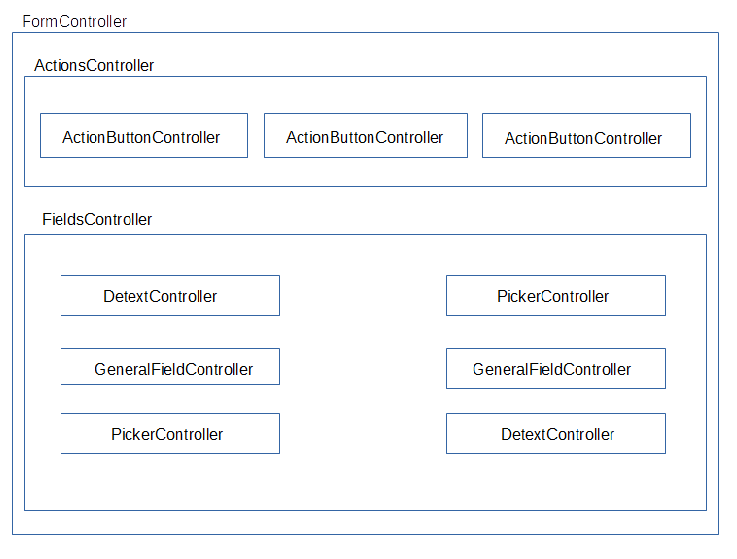
\includegraphics[height=10 cm]{gerarchia-controller}
	\caption{gerarchia di controller in una form}
	\label{fig:ger-contr}
\end{figure}

\section{Validazione dei campi inseriti}

AngularJS mette a disposizione molte funzionalità dedicate alla realizzazione di form.\\
Una di queste è la validazione della form a livello client. AngularJS, in maniera del tutto autmatica, valuta se i dati inseriti siano del tipo dichiarato per ogni campo e se vengono rispettate le obbligatorietà. Un campo viene dichiarato obbligatorio tramite la direttiva \lstinline[language=HTML]!ng-required! \\
La validazione dell'intera form è possibile tramite l'oggetto di sistema \lstinline[language=HTML]!$valid!, una variabile booleana che assume il valore \lstinline[language=HTML]!true! solamente nel caso tutti i campi dati rispettino i vincoli descritti sopra.

\newpage
